\documentclass[a4,landscpae]{seminar}
\pdfcompresslevel=9
\pdfpagewidth=11.69 truein % A4 portrait
\pdfpageheight=8.27 truein % A4 portrait
\pdfhorigin=1truein     % default value(?), but doesn't work without
\pdfvorigin=1truein     % default value(?), but doesn't work without
\slideheight=17.5cm
\slidewidth=23cm

\usepackage[spanish]{babel}
\usepackage[latin1]{inputenc}

\usepackage{t-gsyc-6}
\usepackage{fancybox}
\usepackage{graphics}
\usepackage{moreverb}
\usepackage{alltt}
\usepackage{amsmath}
\usepackage[normalsize]{subfigure}
\usepackage{url}

\title{HACIENDO PROGRAMABLE Y ESTABLE CON FPGA UN DRONE COMERCIAL}
\author{Eloy Navarro Morales}
\conference{Trabajo Fin de Grado}

\cop{E. Navarro}
\begin{document}
\maketitle

%%--------------------------------------------------------------
%% INDICE
%%--------------------------------------------------------------

\begin{hslide}
\slsect{\'Indice}
\begin{itemize}
	\item Introducci\'on
	\item Objetivos
	\item Infraestructura
	\item ...
	\item Conclusiones
\end{itemize}
\end{hslide}

%%--------------------------------------------------------------
%% INTRODUCCION
%%--------------------------------------------------------------

\begin{hslide}
\slsect{Introducci\'on}
\slsubsect{Drones}
\begin{minipage}{6.1cm}
	\begin{figure}
		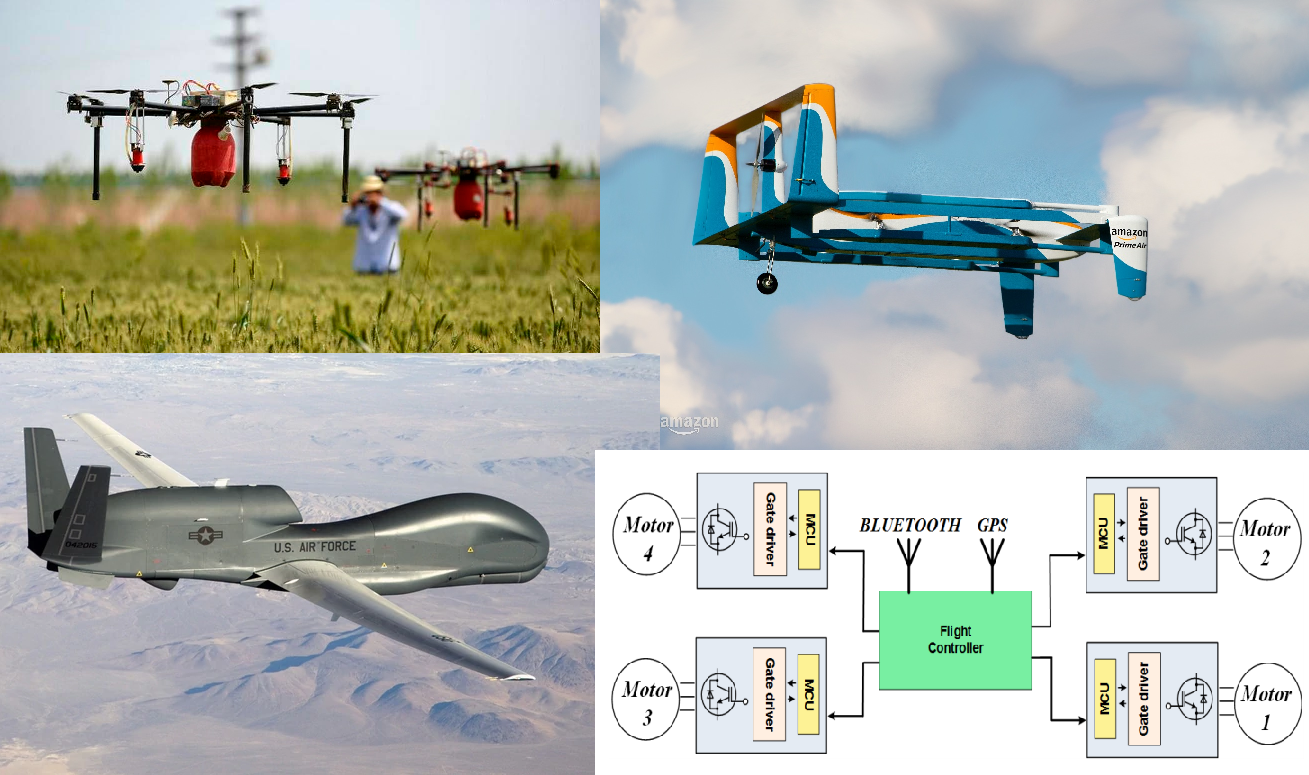
\includegraphics[width=6.2cm]{Imagenes/Intro_Drones}
	\end{figure}
\end{minipage} \hfill
\begin{minipage}{4.9cm}
	\begin{itemize}
		\item Aplicaciones en entorno civil y militar
		\item Sistemas de control variados seg\'un aplicaci\'on
	\end{itemize}
\end{minipage}

\end{hslide}

%%--------------------------------------------------------------

\begin{hslide}
\slsubsect{FPGAs}
\begin{minipage}{7cm}
	\begin{center}
		\begin{figure}
			%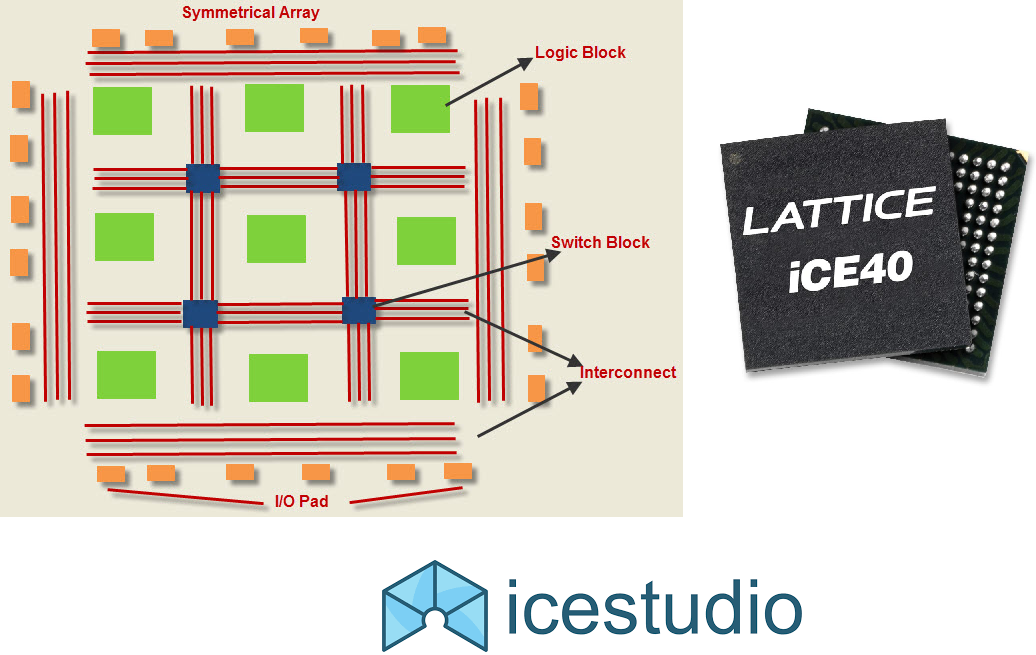
\includegraphics[width=8cm]{Imagenes/Intro_FPGA}
			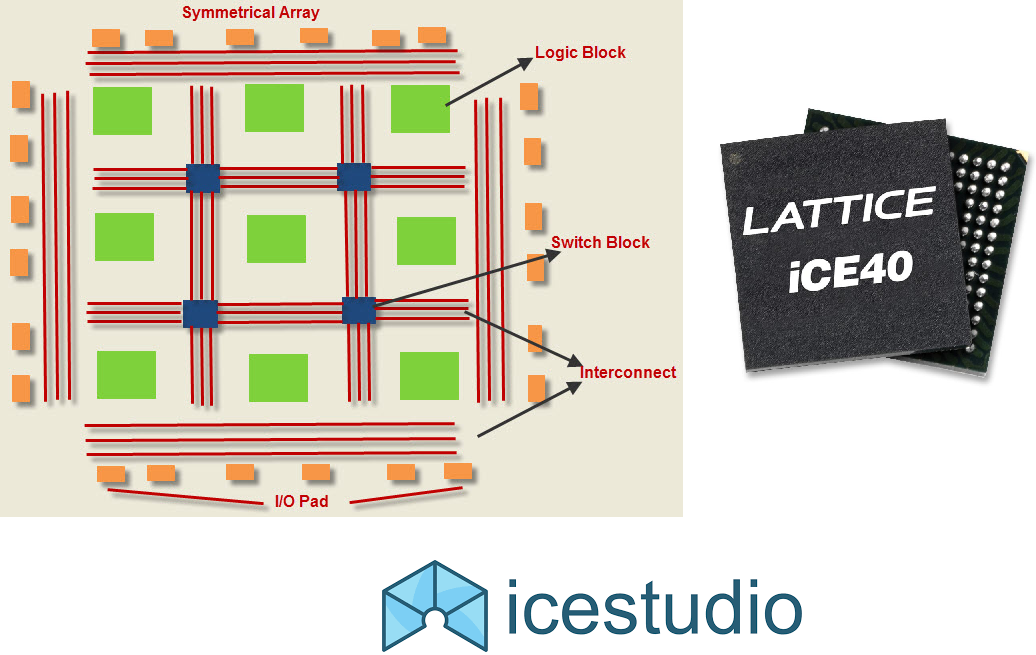
\includegraphics[width=7.5cm]{Imagenes/Intro_FPGA}
		\end{figure}
	\end{center}
\end{minipage} \hfill
\begin{minipage}{3.5cm}
	\begin{itemize}
		\item Potencia paralela
		\item Escalabilidad
		\item Reconfiguraci\'on
		\item Desarrollo abierto
	\end{itemize}
\end{minipage}
\end{hslide}

%%---------------------------------------------------------------


%%---------------------------------------------------------------


%%--------------------------------------------------------------
%% OBJETIVOS
%%--------------------------------------------------------------

\begin{hslide}
\slsect{Objetivos}
Hacer \textbf{estable y programable} el vuelo de un dron comercial de
bajo coste haciendo uso de FPGAs libres

Sub-objetivos:
	\begin{itemize}
		\item Sensorizar veh\'iculo y enlazarlo con tierra
		\item Dise\~nar estaci\'on de tierra y control en comunicaci\'on con dron y PC
		\item Dise\~nar software para PC de mando en Python
	\end{itemize}
\end{hslide}

%%--------------------------------------------------------------

\begin{hslide}
\slsubsect{Requisitos}
	\begin{itemize}
		\item Control en tres grados de libertad independientes
		\item Tiempo real
		\item ... Este apartado quiz\'as sobra?
	\end{itemize}
\end{hslide}

%%--------------------------------------------------------------
%% INFRAESTRUCTURA
%%--------------------------------------------------------------

\begin{hslide}
\slsect{Infraestructura}
\begin{minipage}{6.5cm}
	\slsubsect{Software}
	\begin{itemize}
		\item IDEs: Quartus, IceCube2, ArduinoIDE
		\item Simulaci\'on: ModelSim, FT\_Prog
		\item Programaci\'on y depuraci\'on: Diamond, Logic
	\end{itemize}
	\slsubsect{Hardware}
	\begin{itemize}
		\item Plataformas: Arduino, ICE40, SYMA X5C
		\item Comunicaciones: NRF24L01
		\item Sensores: Flow breakout board

	\end{itemize}
\end{minipage} \hfill
\begin{minipage}{4cm}
	\begin{figure}
		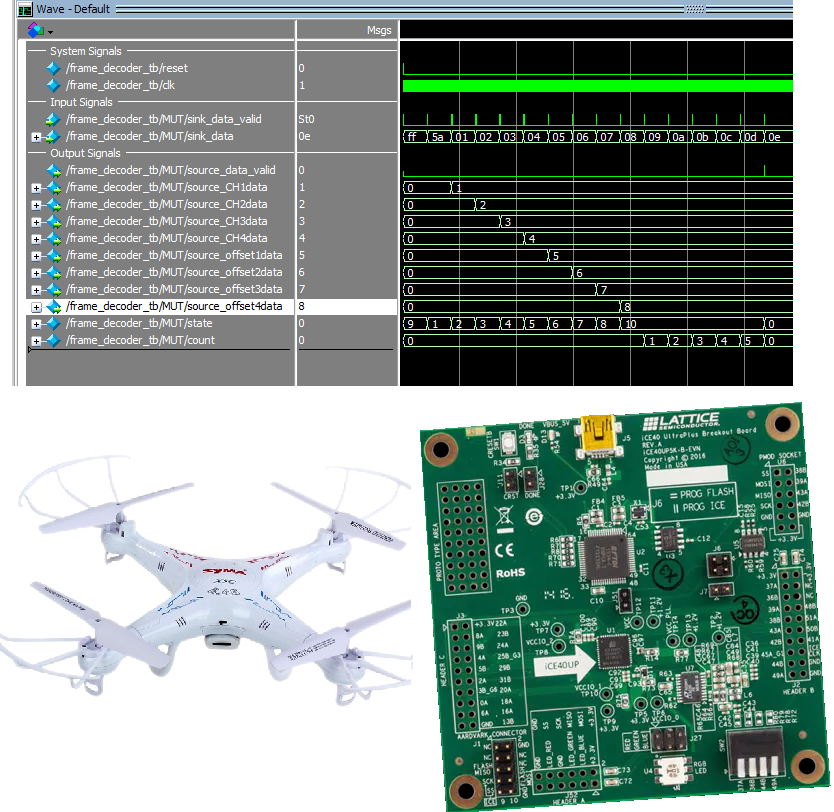
\includegraphics[width=5.2cm]{Imagenes/Infraestructura}
	\end{figure}
\end{minipage} \hfill
\end{hslide}

%%--------------------------------------------------------------


%%---------------------------------------------------------------

\begin{hslide}
\slsubsect{}
\begin{minipage}{5cm}
	\begin{itemize}
		\item M\'as de una foto centrada en lado
	\end{itemize}
\end{minipage} \hfill
\begin{minipage}{2cm}
	\begin{center}
		\begin{figure}
			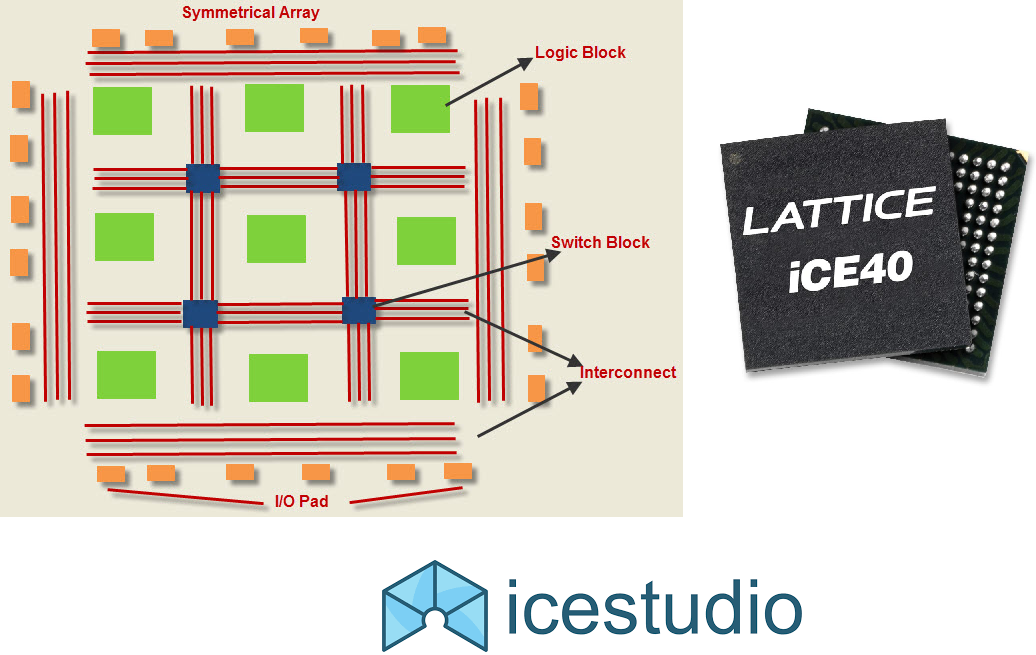
\includegraphics[width=2cm]{Imagenes/Intro_FPGA}
		\end{figure}
	\end{center}
\end{minipage} \hfill
\begin{minipage}{2cm}
	\begin{center}
		\begin{figure}
			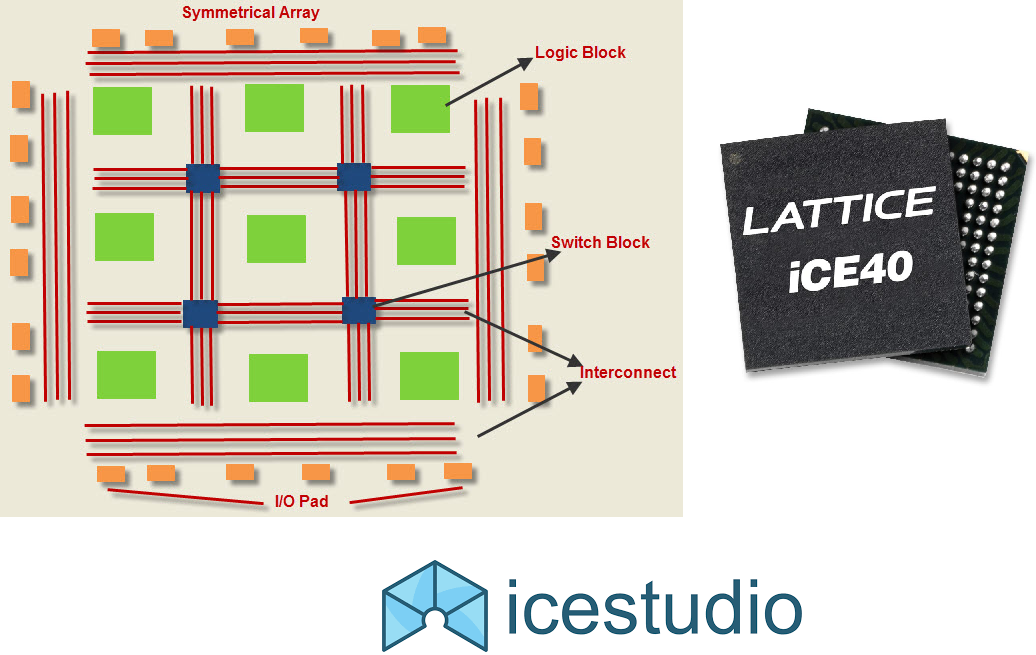
\includegraphics[width=2cm]{Imagenes/Intro_FPGA}
		\end{figure}
	\end{center}
\end{minipage}
\end{hslide}


%%---------------------------------------------------------------

\begin{hslide}
\slsubsect{Anidados}
\begin{minipage}{7cm}
	\begin{itemize}
		\item Nivel 1
		\begin{itemize}
			\item Nivel 2
		\end{itemize}
	\end{itemize}
\end{minipage} \hfill
\end{hslide}

%%---------------------------------------------------------------

\begin{hslide}
\slsubsect{Para c\'odigo - \texttt{aqu\'i}}

\end{hslide}

%%--------------------------------------------------------------

\begin{hslide}
\slsubsect{Experimentos - \texttt{Drone-E010}}

\end{hslide}

%%--------------------------------------------------------------
%% CONCLUSIONES
%%--------------------------------------------------------------

\begin{hslide}
\slsect{Conclusiones y l\'ineas futuras}
\end{hslide}

%%---------------------------------------------------------------

\begin{hslide}
\slsubsect{L\'ineas futuras}

\end{hslide}

%%---------------------------------------------------------------

\end{document}\documentclass[notes,slidesec,a4]{seminar}
